\documentclass[12pt]{article}
\usepackage{graphicx}
\usepackage[margin=30mm, paper = a4paper]{geometry}
\usepackage{minted}
\usepackage{subcaption}
\usepackage{multicol}

\title{Basic MySQL Operations}
\author{Md Tajim An Noor}
\date{}

\begin{document}
\vspace*{\fill}
\begin{center}

    \emph{Heaven's Light is Our Guide} \\
    \textbf{Rajshahi University of Engineering and Technology} \\

    \begin{figure}[h]
        \centering
        
\includegraphics[scale=.34]{images/RUET_logo.png}
        \label{fig:ruet_logo}
    \end{figure}
    \vspace{5mm}

    \textbf{Course Code}\\
    ECE 2216\\
    \vspace{3mm}
    \textbf{Course Title}\\
    Database Systems Sessional

    \vspace{5mm}
    \textbf{Experiment Date:} October 15, 2023,\\
    \textbf{Submission Date:} November 5, 2023\\

    \vspace{5mm}
    \textbf{Lab Report 3:} Creating a database and doing operations on it using SQL\\

    \vspace{15mm}

    \begin{tabular}{c|c}
        \textbf{Submitted to} & \textbf{Submitted by} \\
        Md. Robiul Islam      & Md. Tajim An Noor     \\
        Assistant Professor   & Roll: 2010025         \\
        Dept of ECE, Ruet     &                       \\
    \end{tabular}

\end{center}
\vspace*{\fill}

\pagebreak

\tableofcontents

\maketitle

\section{Tools Used}
\begin{itemize}
    \item MySQL
    \item VS Code - as an IDE to use SQL
    \item MacTeX -\LaTeX  compiler
    \item VS Code with LaTeX workshop extension as a text editor
\end{itemize}


\section{Process}
The task is to create a database and then do some operations on the database using the SELECT, WHERE, LIKE, IN operator.

\subsection{SQL Codes:}
Create a table, order\_details(order\ code, customer\ name, mobile, address, product\ ordered, category, quantity, delivery\ status, remark)
\subsubsection*{Code:}
\begin{minted}[breaklines, linenos]{mysql}
CREATE DATABASE IF NOT EXISTS ProductOrderDetailsLR3;
-- creating databse
-- creating the table as instructed
CREATE TABLE ProductOrderDetailsLR3.Order_Details(
    order_code int Auto_Increment Primary Key,
    customer_name varchar(30),
    mobile varchar(30),
    address_ varchar(70),
    product_ordered varchar(30),
    catagory varchar(30),
    quantity int,
    delivery_status boolean,
    remark varchar(40)
)
\end{minted}
\vspace{10mm}

\subsubsection{Add two columns order date and delivered date into the table.}
\subsubsection*{Code: }
\begin{minted}[breaklines, linenos]{mysql}
alter TABLE
ProductOrderDetailsLR3.Order_Details
ADD
    order_date date,
ADD
    delivery_date date;
\end{minted}

\vspace{13mm}

\subsubsection{Insert values into the table where number of row  is at least 15.}
\subsubsection*{Code: }
\begin{multicols*}{2}
    \begin{minted}[breaklines, breakanywhere, linenos]{mysql}
INSERT INTO 
ProductOrderDetailsLR3.
Order_Details
    (
        customer_name,
        mobile,
        address_,
        product_ordered,
        catagory,
        quantity,
        delivery_status,
        remark,
        order_date,
        delivery_date
    )
VALUES
    (
        'Rifath',
        '016245226784',
        'Vataopara, Lokkhipur, Rajshahi',
        'Mechanical Keyboard',
        'Tech Accessories',
        1,
        '1',
        'Good customer',
        '2023-06-11',
        '2023-06-14'
    ),
    (
        'Sazid',
        '01828798623',
        'Zia Hall, RUET',
        'Freeze',
        'Home Appliance', 
        1,
        '1',
        'Borolox customer',
        '2023-01-01',
        '2023-02-14'
    )...
\end{minted}
    To save space only two instances of the input values are shown.
\end{multicols*}


\vspace{13mm}

\subsubsection{Find the customers who have ordered from Rajshahi.}
\subsubsection*{Code:}

\begin{minted}[breaklines, linenos]{mysql}
SELECT
    customer_name as Customer_Name,
    address_ as Ordered_From
FROM
    ProductOrderDetailsLR3.Order_Details
where
    address_ like '%Rajshahi%'
\end{minted}



\vspace{13mm}

\subsubsection{Find the customers and their full address whose order has been canceled with a remark of "can not be processed".}
\subsubsection*{Code:}
\begin{minted}[breaklines, linenos]{mysql}
-- updating the remarks as Cannon be proccessed for future operations
UPDATE
    ProductOrderDetailsLR3.Order_Details
set
    remark = 'Cannot be proccessed'
WHERE
    delivery_status = 0
-- finding the customers
SELECT
    customer_name as Customer_Name,
    address_ as Ordered_From
FROM
    ProductOrderDetailsLR3.Order_Details
where
    remark = 'Cannot be proccessed'
\end{minted}

\vspace{13mm}
\pagebreak
\subsubsection{Find the customers and product they ordered who have ordered after "30-10-2021"}
\subsubsection*{Code:}
\begin{minted}[breaklines, linenos]{mysql}
SELECT
    customer_name as Customer_Name,
    product_ordered as Product
FROM
    ProductOrderDetailsLR3.Order_Details
where
    order_date > '2021-10-30'
\end{minted}

\vspace{13mm}

\subsubsection{Find the order code and customer's mobile who ordered 5, 10 or 15 numbers of products.}
\subsubsection*{Code:}
\begin{minted}[breaklines, linenos]{mysql}
SELECT
    order_code as Order_Code,
    mobile as Customer_Mobile,
    quantity
FROM
    ProductOrderDetailsLR3.Order_Details
WHERE
    quantity in(5, 10, 15)
\end{minted}

\vspace{13mm}

\section{Output}
\captionsetup{justification=centering}
\begin{figure}[htbp!]
    \begin{subfigure}{1\textwidth}
        \centering
        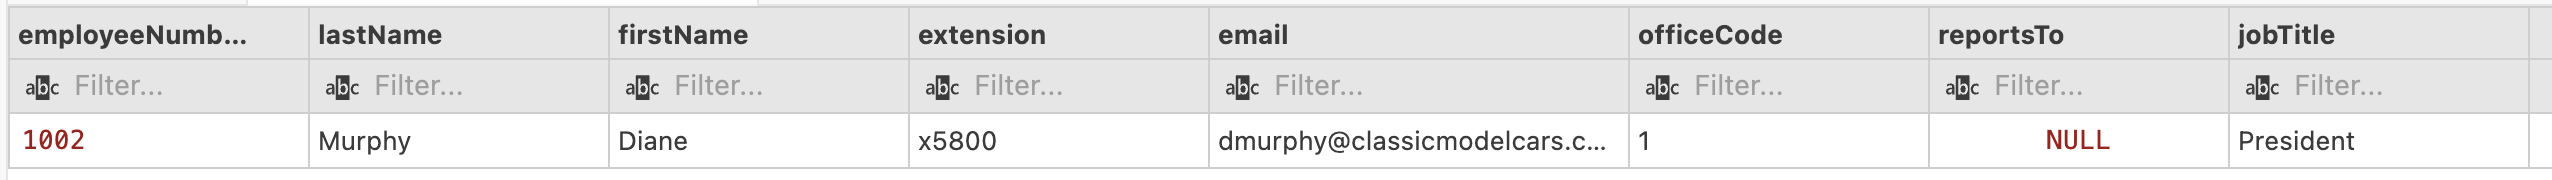
\includegraphics[width=\linewidth]{images/output/q1.png}
        \caption*{The person who is the top of the organization (i.e. reports to no one)}
        \label{fig:q1}
    \end{subfigure}
    \vspace*{20mm}
    \begin{subfigure}{.3\textwidth}
        \centering
        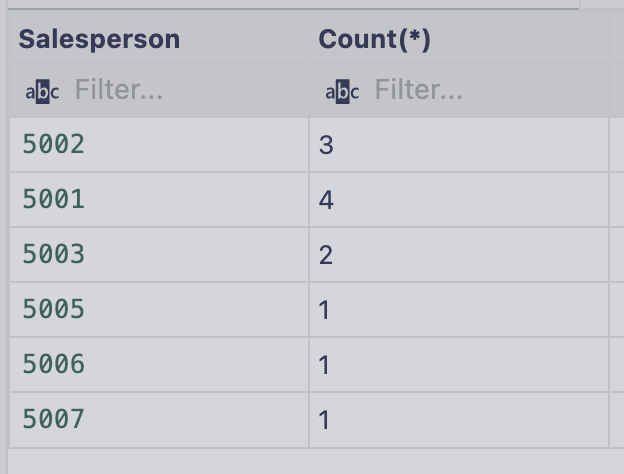
\includegraphics[width=.6\linewidth]{images/output/q2.png}
        \caption*{Difference in days between the most recent and oldest order date in Orders file.}
        \label{fig:q2}
    \end{subfigure}
    \begin{subfigure}{.3\textwidth}
        \centering
        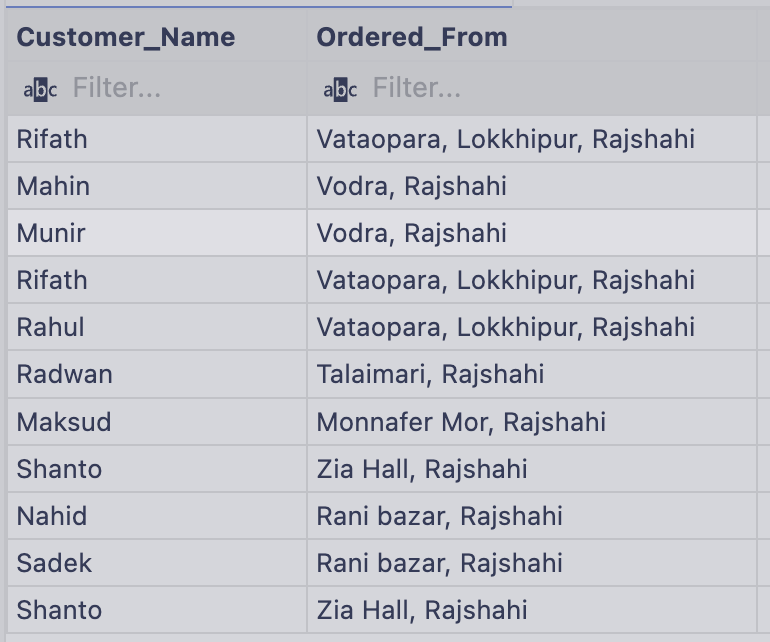
\includegraphics[width=.6\linewidth]{images/output/q3.png}
        \caption*{Total value of  payments received in July 2004.}
        \label{fig:q3}
    \end{subfigure}
    \begin{subfigure}{.3\textwidth}
        \centering
        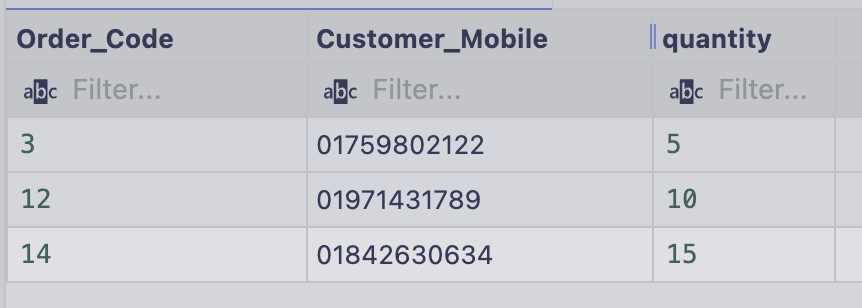
\includegraphics[width=.6\linewidth]{images/output/q6.png}
        \caption*{The number of orders ‘On Hold’ for each customer.}
        \label{fig:q6}
    \end{subfigure}

    \begin{subfigure}{\textwidth}
        \centering
        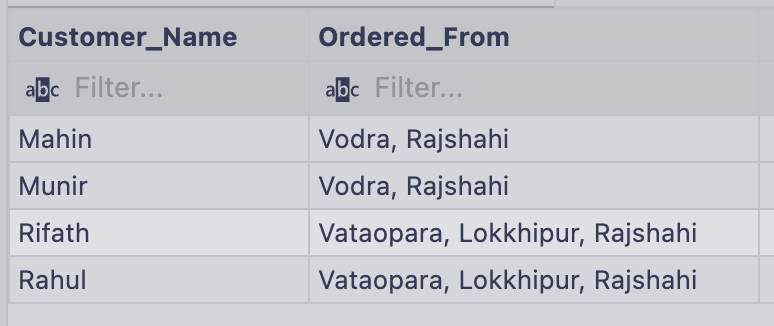
\includegraphics[width=.5\linewidth]{images/output/q4.png}
        \caption*{Profit generated by each sales representative based on the orders from the customers they serve. Sorted by profit generated descending.}
        \label{fig:q4}
    \end{subfigure}
    \begin{subfigure}{.5\textwidth}
        \centering
        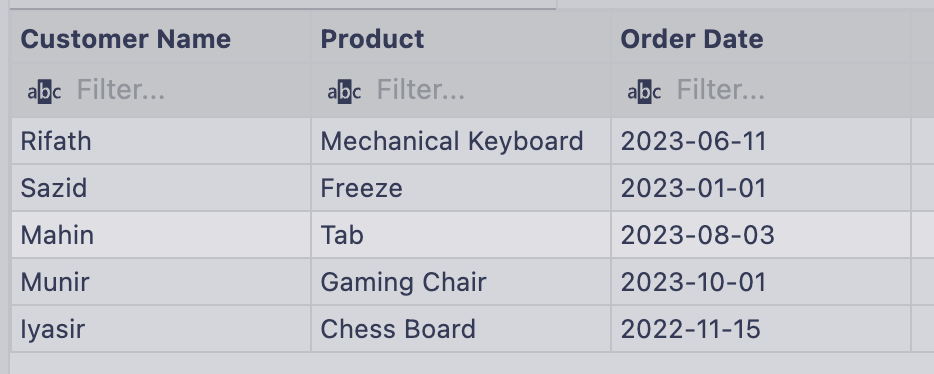
\includegraphics[width=.8\linewidth]{images/output/q5.png}
        \caption*{Products sold in 2003 but not 2004.}
        \label{fig:q5}
    \end{subfigure}
    \begin{subfigure}{.5\textwidth}
        \centering
        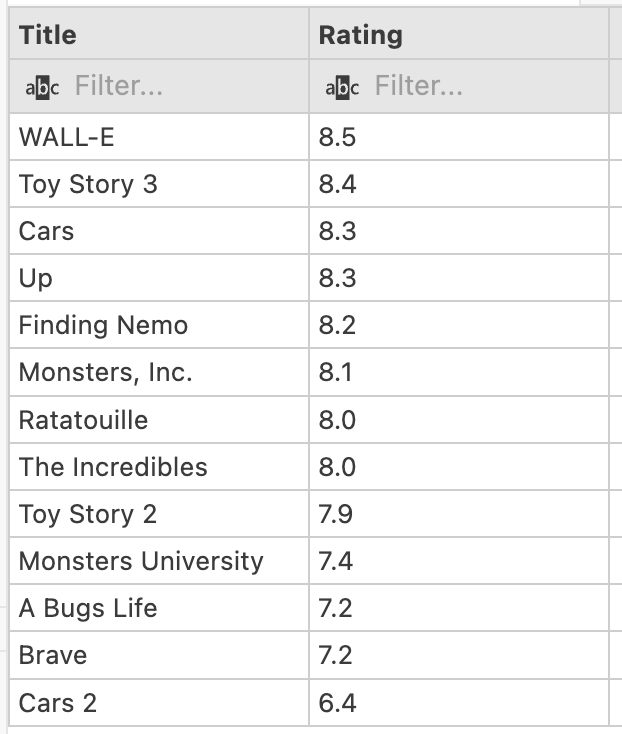
\includegraphics[width=.65\linewidth]{images/output/q7.png}
        \caption*{Names of products sold at less than 80\% of the MSRP.}
        \label{fig:q7}
    \end{subfigure}
\end{figure}


\end{document}